% !TeX root = Bericht_main.tex

\subsection{Aufgabe 31}

In Aufgabe 31 versuchen wir Schritt für Schritt eine sinnvolle Wahl für die Feinheit von Orts- bzw. Zeitdiskretisierung herauszufinden. Dazu ermitteln wir abhängig vom Verfeinerungslevel $level = 0,1,2$ eine sinnvolle Zeitschrittweite, sodass der Fehler der Zeitdiskretisierung kleiner als der Ortsfehler ist und der Startwert des Newton-Verfahrens so gut ist, dass die Newton-Konvergenz quadratisch ist. 
Wir vergleichen dazu die Masse der Konzentration in einem Plot für das exponentielle Wachstum mit $ Reaction = 2.5 $

\begin{figure}[H]
	\centering
	\captionabove{Vergleich der Masse für unterschiedliche Zeitdiskretisierungen}
	\subfigure[auf Level = 0]{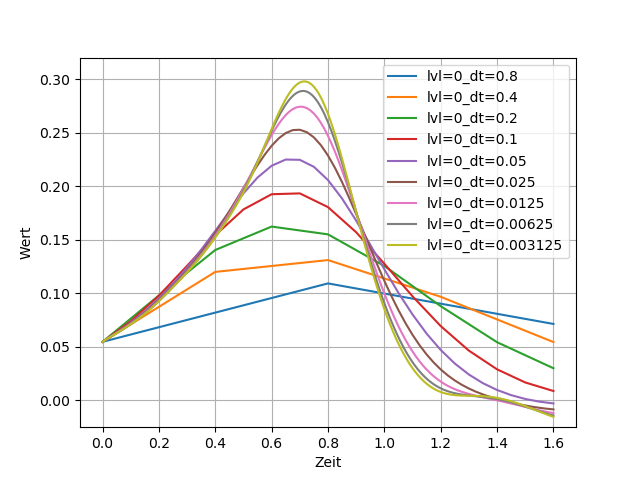
\includegraphics[width=0.85\textwidth]{../Aufgabe31/Maxdiff/zeitvergleich_lvl=0_plot.png}}
\end{figure}
\begin{figure}[H]
	\centering
	\subfigure[auf Level = 1]{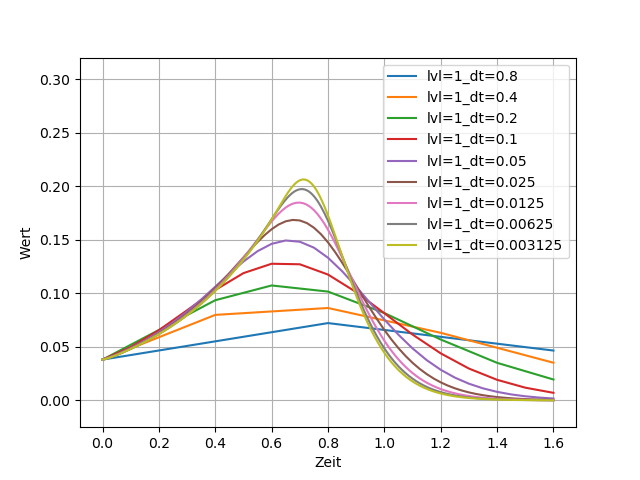
\includegraphics[width=0.85\textwidth]{../Aufgabe31/Maxdiff/zeitvergleich_lvl=1_plot.png}}
\end{figure}
\begin{figure}[H]
	\centering
	\subfigure[auf Level = 2]{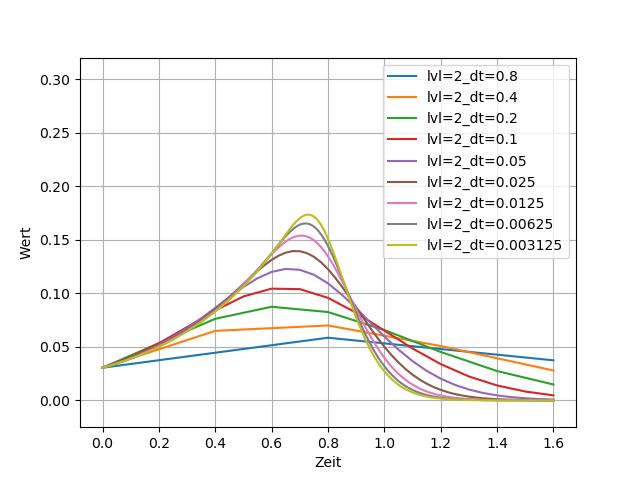
\includegraphics[width=0.85\textwidth]{../Aufgabe31/Maxdiff/zeitvergleich_lvl=2_plot.png}}
\end{figure}

Um zusätzlich zum Fehler der Zeitdiskretisierung auch den Fehler der Ortsdiskretisierung abschätzen zu können, ist es zudem hilfreich auch die verschiedenen Masseplots für eine fest gewählte Zeitdiskretisierung auf den unterschiedlichen Levels zu vergleichen:
 
 \begin{figure}[H]
 	\centering
 	\captionabove{Vergleich der Masse für $Level = 1,2,3$}
 	\subfigure[mit $dt = 0.8$]{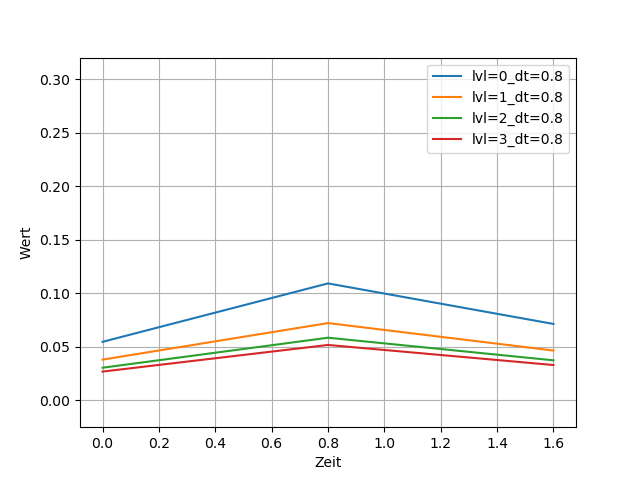
\includegraphics[width=0.32\textwidth]{../Aufgabe31/Maxdiff/3vergleich_dt=08_plot.png}}
 	\subfigure[mit $dt = 0.4$]{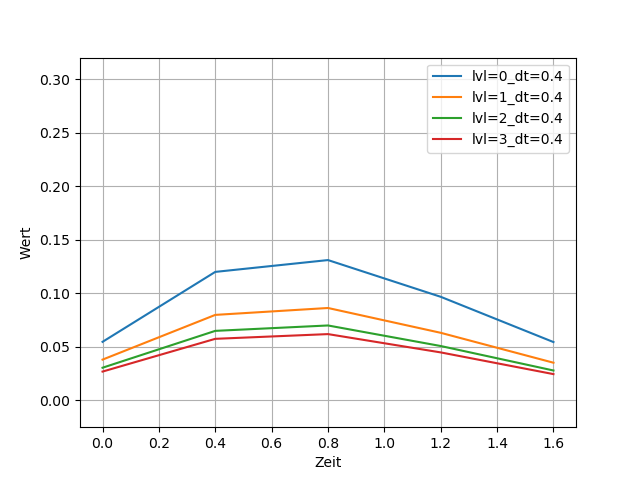
\includegraphics[width=0.32\textwidth]{../Aufgabe31/Maxdiff/3vergleich_dt=04_plot.png}}
 	\subfigure[mit $dt = 0.2$]{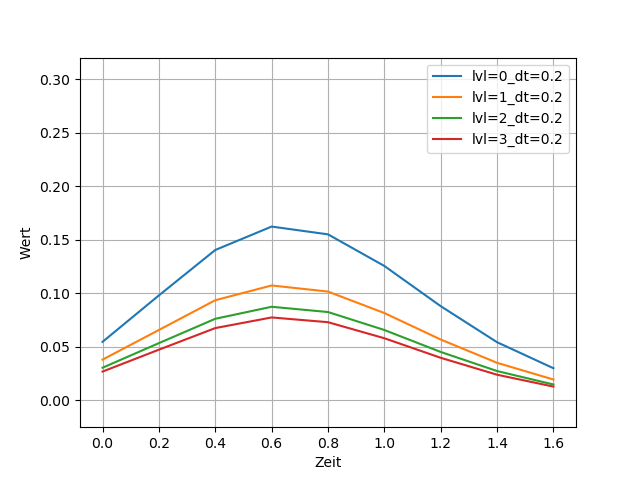
\includegraphics[width=0.32\textwidth]{../Aufgabe31/Maxdiff/3vergleich_dt=02_plot.png}}
 	\subfigure[mit $dt = 0.1$]{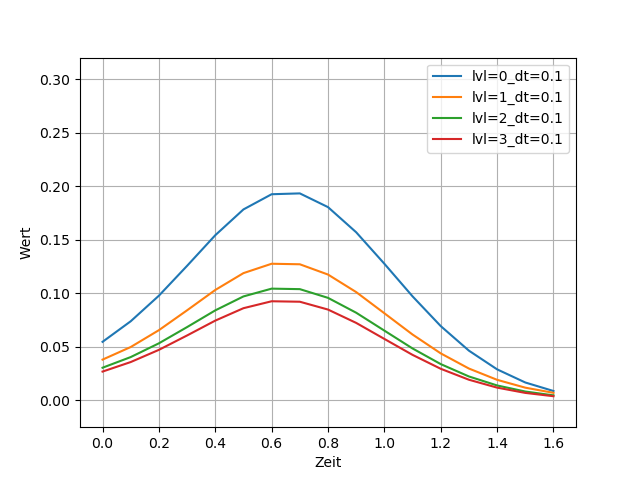
\includegraphics[width=0.32\textwidth]{../Aufgabe31/Maxdiff/3vergleich_dt=01_plot.png}}
 	\subfigure[mit $dt = 0.05$]{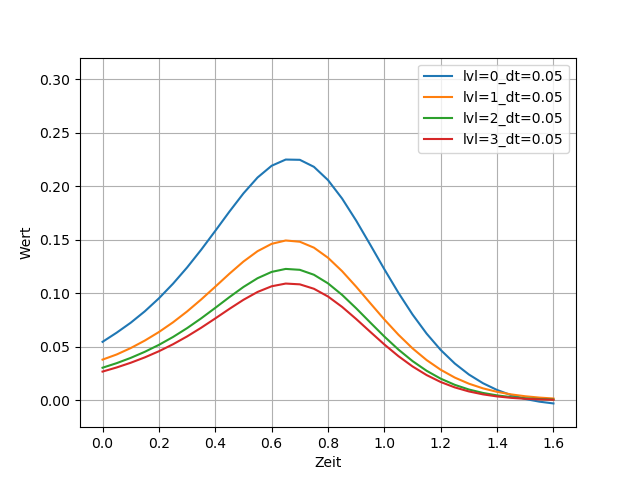
\includegraphics[width=0.32\textwidth]{../Aufgabe31/Maxdiff/3vergleich_dt=005_plot.png}}
 	\subfigure[mit $dt = 0.025$]{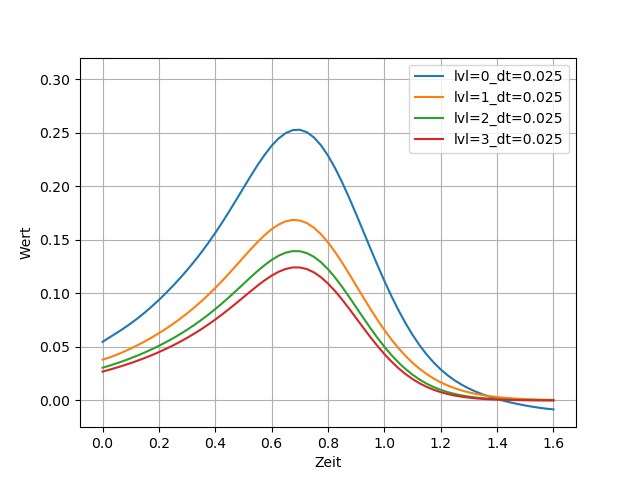
\includegraphics[width=0.32\textwidth]{../Aufgabe31/Maxdiff/3vergleich_dt=0025_plot.png}}
 	\subfigure[mit $dt = 0.0125$]{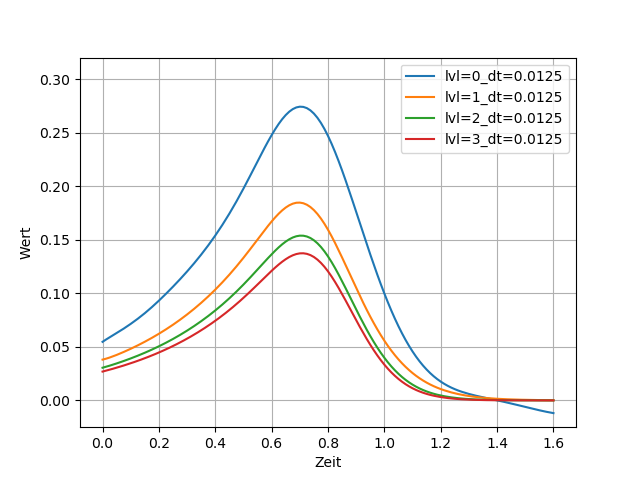
\includegraphics[width=0.32\textwidth]{../Aufgabe31/Maxdiff/3vergleich_dt=00125_plot.png}}
 	\subfigure[mit $dt = 0.00625$]{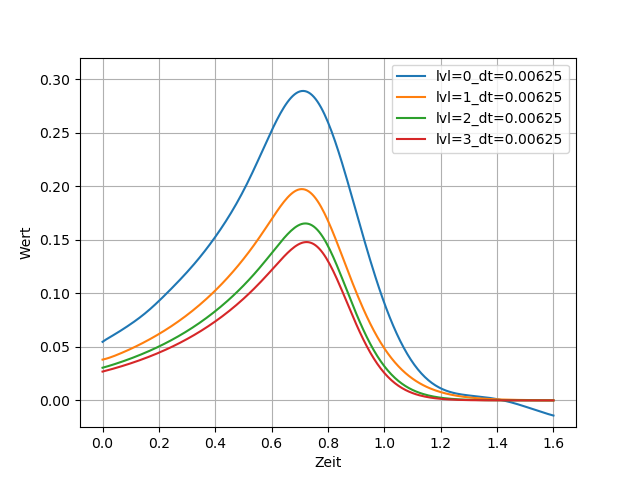
\includegraphics[width=0.32\textwidth]{../Aufgabe31/Maxdiff/3vergleich_dt=000625_plot.png}}
 \end{figure}

Ziel ist es nun, die Fehler der Zeit- bzw. Orstdiskretisierung für für ein bestimmtes Level mit einer bestimmten Schrittweite zu schätzen. 
Dazu vergleichen wir für den Ortsfehler die Masse der aktuellen Zeitschrittweite und des aktuellen Levels mit der Masse der aktuellen Zeitschrittweite und des nächstfeineren Levels.
Für den Fehler der Zeitdiskretisierung vergleichen wir die Masse der aktuellen Zeitschrittweite und des aktuellen Levels mit der Masse des aktuellen Levels und der nächstfeineren Zeitschrittweite.
Als erste Annäherung an eine Metrik betrachten wir jeweils den maximalen Unterschied der einzelnen Massewerte zu den verschiedenen Zeitschritten $t$.
Bei dem Fehler der Ortsdiskretisierung lassen wir, wie oben beschrieben, die Zeitschrittweite fest und erhalten so für genau dieselben Zeitschritte $t$ entsprechende Massewerte. Somit erhalten wir 
\begin{align*}
	r_{Ort}  \approx \max_{t \in \{t_0 = 0,t_1,...,t_n=1.6 \}  } |m_{lvl}(t) - m_{lvl + 1} (t) |
\end{align*}
Bei dem Fehler der Zeitdiskretisierung haben wir zwar bei der feineren Schrittweite theoretisch mehr Werte zu Verfügung, wir vergleichen aber auch hier nur an den Zeitschritten $t$ der gröberen Schrittweite, da wir sonst die Zwischenwerte interpolieren müssten:
\begin{align*}
r_{Zeit}  \approx \max_{t \in \{t_0 = 0,t_1,...,t_n=1.6 \}  } |m_{dt}(t) - m_{dt/2} (t) |
\end{align*}
Wir erhalten so folgende Werte als Heatmap:
\begin{figure}[H]
	\centering
	\captionabove{Annäherungen an Fehler der Zeit- und Ortsdiskretisierung}
	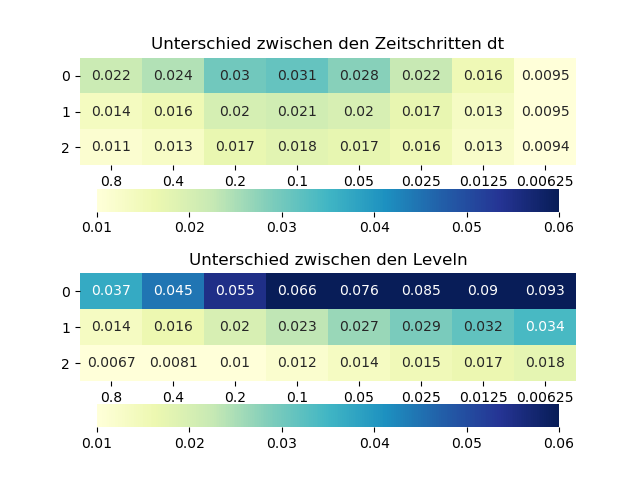
\includegraphics[width=0.85\textwidth]{../Aufgabe31/Maxdiff/Heatmapblub.png}
\end{figure}
Dabei sind die Werte in 'Unterschied zwischen den Zeitschrittschritten' gerade der oben erklärte Wert $r_{Zeit}$ und die Werte in  'Unterschiede zwischen den Leveln' gerade der Wert $r_{Ort}$

Damit können wir folgende sinnvolle Werte für die Zeitschrittweite herauslesen:
\begin{figure}[H]
	\centering
	\captionabove{Sinnvolle Werte für die Zeitschrittweite abhängig vom Level}
	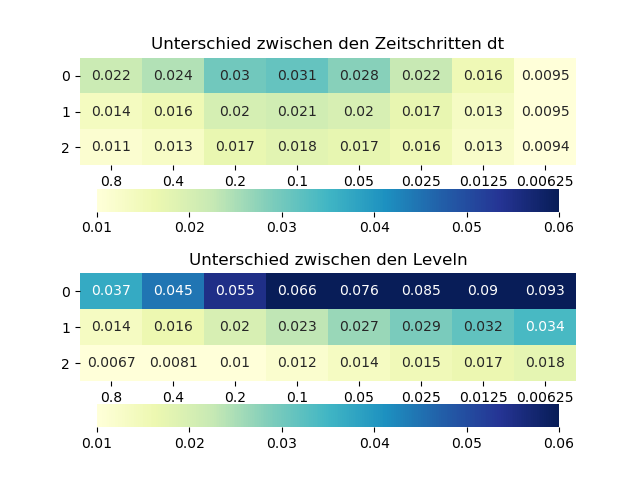
\includegraphics[width=0.85\textwidth]{../Aufgabe31/Maxdiff/Heatmapblub1.png}
\end{figure}
Für Level 0  reicht uns bereits die geringste Zeitschrittweite $dt = 0.8$, anders ausgedrückt, der Fehler der Orstdiskretisierung ist schlichtweg zu groß. Für Level 1 erhalten wir $dt= 0.1$ als sinnvolle Wahl, denn für eine geringere Zeitschrittweite überwiegt der Fehler der Orstdiskretisierung, für eine größere Wahl von dt ist hingegen der Fehler der Zeitdiskretisierung nicht mehr kleiner als der Fehler der Fehler der Orstdiskretisierung.
Nach analogem Auswahlverfahren erhalten wir für Level 2 $dt = 0.0125$ als sinnvolle Wahl für die Zeitschrittweite.
\newline
Diese Ergebnisse ließen sich auch für andere "Metriken" nachvollziehen.
So versuchten wir uns anschließend an der L2-Norm. Zunächst müssen wir dazu die Massewerte interpolieren, dazu wählen wir (für $dt = 0.8$ quadratische, ansonsten) kubische Splines. Anschließend erhielten wir den Fehler der Orts- /Zeitdiskretisierung wie folgt:
\begin{align*}
r_{Ort}  &\approx \int_0^{1.6} |f_{m_{lvl}}(t) - f_{m_{lvl + 1}}  (t) |^2 dt  \\
r_{Zeit}  &\approx \int_0^{1.6}  |f_{m_{dt}}(t) - f_{m_{dt/2} }(t) |^2 dt
\end{align*}
dabei bezeichne $f_{m_{  \star }}$ jeweils die Interpolationsfunktion zu den entsprechenden Massewerten (vgl. die Erklärungen dazu weiter oben).
Wir erhalten so: 
\begin{figure}[H]
	\centering
	\captionabove{Annäherungen an Fehler der Zeit- und Ortsdiskretisierung durch L2-Norm}
	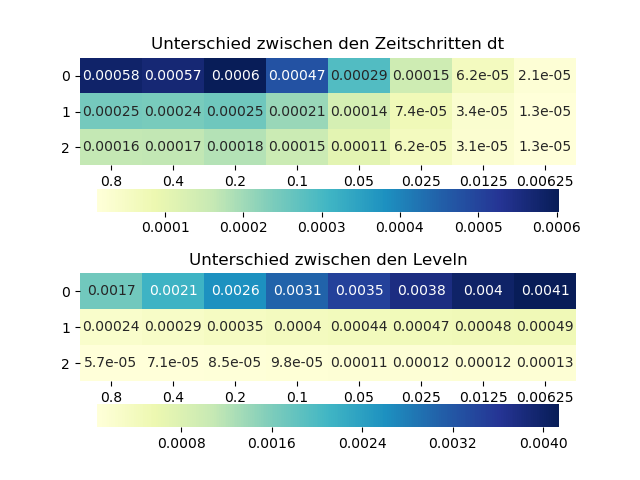
\includegraphics[width=0.85\textwidth]{../Aufgabe31/Maxdiff/Heatmapblubintegral.png}
\end{figure}
Dabei finden wir erneut, wenn auch nichtmehr ganz so eindeutig, unsere oben ermittelten Werte für sinnvolle Zeitschrittweiten abhängig vom Level:
\begin{figure}[H]
	\centering
	\captionabove{Resultierende sinnvolle Werte für die Zeitschrittweite abhängig vom Level}
	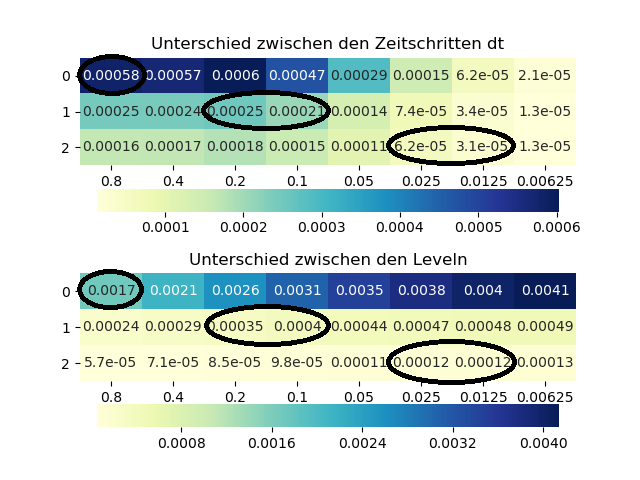
\includegraphics[width=0.85\textwidth]{../Aufgabe31/Maxdiff/Heatmapblubintegral1.png}
\end{figure}
Zur Erinnerung, wir hatten als sinnvolle Werte ermittelt:
\begin{itemize}
	\item Für Level 0: \qquad $dt = 0.8$ (Ortsfehler einfach zu groß)
	\item Für Level 1: \qquad $dt = 0.1$ 
	\item Für Level 2: \qquad $dt = 0.0125$
\end{itemize}
 




